\documentclass[tikz,border=8pt]{standalone}
\usepackage{pgfplots}
\pgfplotsset{compat=1.18}
\definecolor{chapterteal}{HTML}{196F6B}
\definecolor{chapterrust}{HTML}{A3472F}
\definecolor{chaptergold}{HTML}{C58B18}
\definecolor{chapterblue}{HTML}{174F75}

\begin{document}

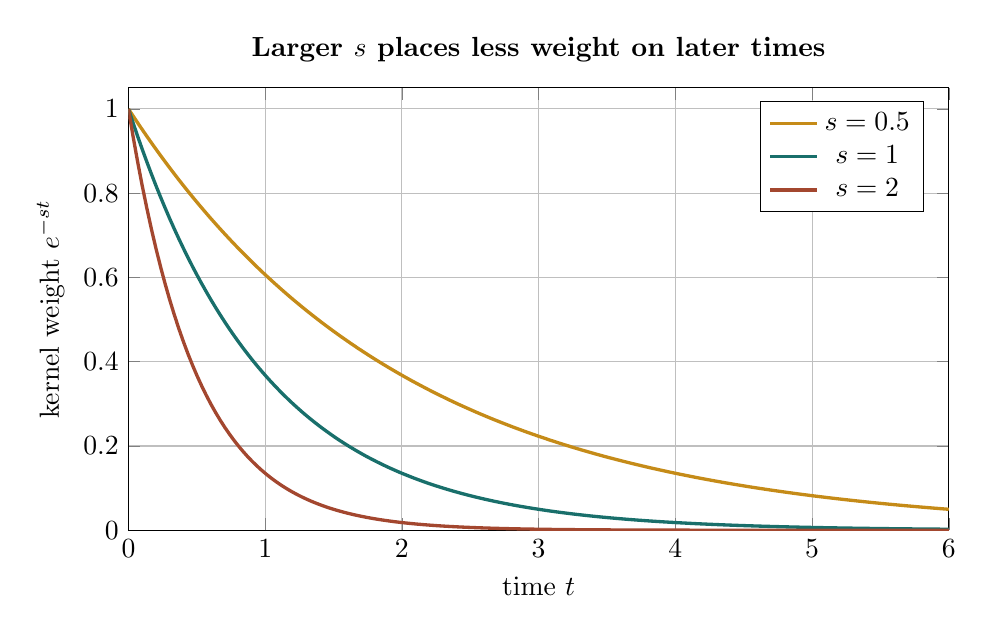
\begin{tikzpicture}
\begin{axis}[
  width=12cm,
  height=7.2cm,
  xmin=0,xmax=6,
  ymin=0,ymax=1.05,
  xlabel={time $t$},
  ylabel={kernel weight $e^{-st}$},
  title={Larger $s$ places less weight on later times},
  title style={font=\bfseries},
  grid=both,
  legend pos=north east,
  samples=180,
  domain=0:6
]
\addplot[chaptergold,very thick] {exp(-0.5*x)};
\addlegendentry{$s=0.5$}
\addplot[chapterteal,very thick] {exp(-x)};
\addlegendentry{$s=1$}
\addplot[chapterrust,very thick] {exp(-2*x)};
\addlegendentry{$s=2$}
\end{axis}
\end{tikzpicture}

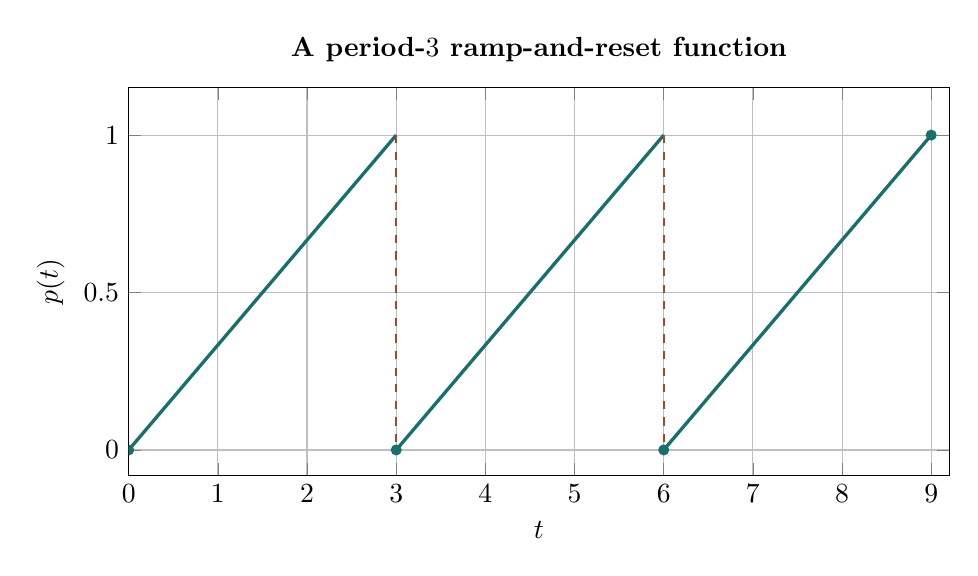
\begin{tikzpicture}
\begin{axis}[
  width=12cm,
  height=6.5cm,
  xmin=0,xmax=9.2,
  ymin=-0.08,ymax=1.15,
  xlabel={$t$},
  ylabel={$p(t)$},
  title={A period-$3$ ramp-and-reset function},
  title style={font=\bfseries},
  grid=both,
  xtick={0,1,2,3,4,5,6,7,8,9},
  ytick={0,0.5,1}
]
\addplot[chapterteal,very thick] coordinates {(0,0) (3,1)};
\addplot[chapterteal,very thick] coordinates {(3,0) (6,1)};
\addplot[chapterteal,very thick] coordinates {(6,0) (9,1)};
\addplot[chapterrust,dashed,thick] coordinates {(3,1) (3,0)};
\addplot[chapterrust,dashed,thick] coordinates {(6,1) (6,0)};
\fill[chapterteal] (axis cs:0,0) circle (2pt);
\fill[chapterteal] (axis cs:3,0) circle (2pt);
\fill[chapterteal] (axis cs:6,0) circle (2pt);
\fill[chapterteal] (axis cs:9,1) circle (2pt);
\end{axis}
\end{tikzpicture}

\end{document}
